\section{Reducing the size of the Petri net in postprocessing}
\label{sec:future-work-petri-net-reduction}

\cite{murata1989} describes in a Section titled ``Simple Reduction Rules for Analysis''
six operations that preserve the properties of safeness, liveness, and boundedness of \acrshort{PN}.
See Definitions \ref{definition:safeness}, \ref{definition:liveness} and \ref{definition:boundedness}
respectively for a refresher of what these properties mean.

The six operations involve simplifications that reduce the number of places or transitions
in the Petri net. Next, we reproduce the names used for the reduction rules in the paper and
Fig. \ref{fig:petri-net-reduction-rules} depicts the transformation that takes place in each case.

\begin{enumerate}[label={\alph*)}]
  \item Fusion of Series Places.
  \item Fusion of Series Transitions.
  \item Fusion of Parallel Places.
  \item Fusion of Parallel Transitions.
  \item Elimination of Self-Loop Places.
  \item Elimination of Self-Loop Transitions.
\end{enumerate}

\begin{figure}[!htb]
  \centering
  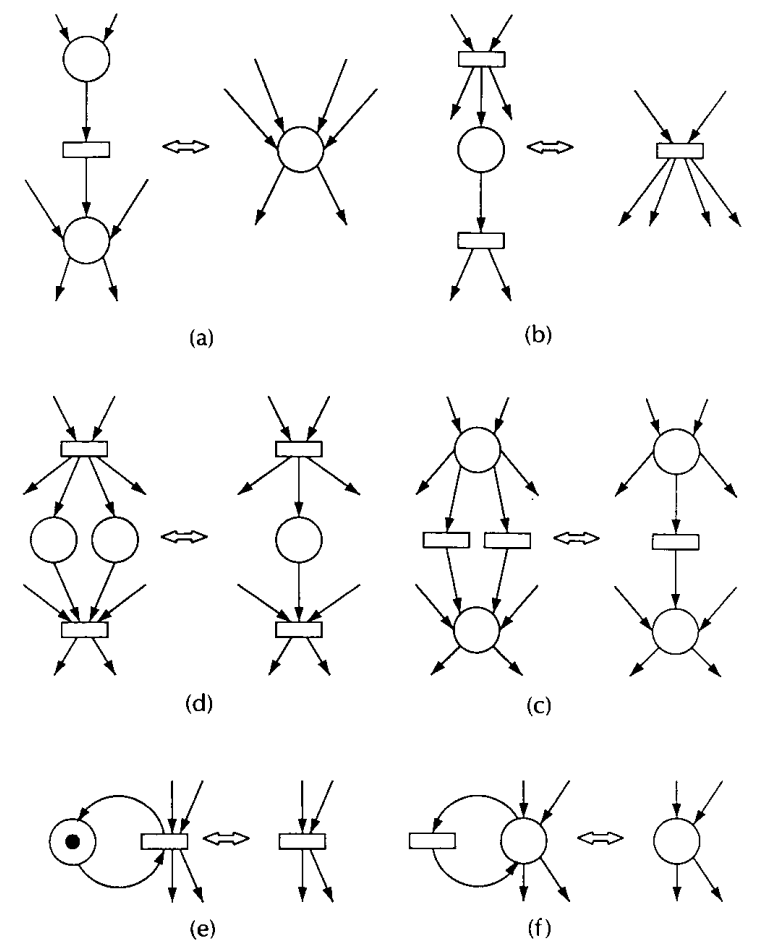
\includegraphics[width=0.9\linewidth]{petri-net-reduction-rules.png}
  \caption{The reduction rules presented in Murata's paper.}
  \label{fig:petri-net-reduction-rules}
\end{figure}

As these operations do not impact the liveness property,
the outcome of the deadlock detection remains unchanged.
Consequently, it might be advantageous to reduce the size of the \acrshort{PN}
after the translation process using specific methods available in the \Rustinline{netcrab} library.
This step should be performed after translating all threads but before invoking the model checker.

Incorporating this functionality into the \acrshort{PN} library itself would be more suitable,
as it would allow other applications to benefit from this feature.
It would be interesting to investigate whether
this approach proves helpful when translating larger programs
that contain hundreds or thousands of places and transitions.

One notable drawback of applying these operations is
that it could obscure the source of the deadlock.
It is valuable for the user to have precise information
about the line in the source code where the deadlock occurs.
If the corresponding transitions or places representing this line are merged,
this information is lost.
However, this disadvantage may be deemed acceptable when dealing with extensive models,
and the feature could be enabled or disabled at the discretion of the user.

\section{Eliminating the cleanup paths from the translation}
\label{sec:future-work-no-cleanup}

The error handling mechanism in the \acrshort{MIR}
must account for every possible scenario of failure during runtime.
The aim of the \emph{rustc} compiler is to ensure
that compiled code fails gracefully,
even in the most extreme circumstances,
e.g., when the program is running out of memory or system calls fail unexpectedly
due to hard limits on the resources available or other causes.
However, the majority of this safeguarding cleanup code is never executed in practice.
\acrshort{OOM} errors and \acrshort{OS} failures are uncommon
and if they indeed emerge, a deadlock in user code is the least of our problems.

\cite{meyer2020} argues that
the program will always terminate in a panic end-state
once a single function call or assertion fails.
Instead of translating the alternative path that the execution follows in the MIR,
he proposes to set a token in the place \Rustinline{PROGRAM_PANIC} directly.
This is equivalent to ignoring the specific cleanup target \acrshort{BB}
during the translation process
and connecting the \acrshort{BB} to the \Rustinline{PROGRAM_PANIC} place
as if it were an \Rustinline{Unwind} terminator (Sec. \ref{sec:terminators}).

This reduces the size of the Petri net model substantially.
It comes with the disadvantage that cleanup \acrshort{BB} are visited but never connected
to other \acrshort{BB}.
These must be removed in a postprocessing step to not clutter the final model.
Meyer's implementation does not seem to have performed this crucial step.
It is unclear whether the implementation matches what the thesis proposed because
the source code cannot be compiled anymore and no output examples are present in the
repository\footnote{\url{https://github.com/Skasselbard/Granite}}.

The claim that the panic state is unrecoverable necessitates thorough examination,
as we have previously observed in the introduction to Rust
that the programmer has the option to utilize \Rustinline{std::panic::catch_unwind}.
Furthermore, this intuitive reasoning might overlook situations
in which a deadlock arises following a panic.
This need not be a catastrophic failure.
Consider for instance a thread that deadlocks while waiting on a message
from another thread that panicked due to incorrect user input.

In conclusion, this modification of the translation logic looks promising
to significantly reduce the number of places and transitions in the \acrshort{PN},
especially in larger models, but more research is needed.

\section{Translated function cache}
\label{sec:future-work-function-cache}

A cache that stores functions after translating them is
an interesting optimization to explore.
The goal is to avoid redundant translations of the same function
when it is called multiple times within the program.
This idea was already briefly mentioned (but not implemented) in \cite{meyer2020}.
The current implementation does not incorporate such caching mechanisms.

This cache would have to store a separate \acrshort{PN} for each function.
It could be realized as a \Rustinline{HashMap<rustc_hir::def_id::DefId, PetriNet>},
analogous to the function counter already present in the implementation.
Furthermore, the translation process would need to merge/connect
the Petri nets resulting from each translated function.
This merging step requires support from the \acrshort{PN} library \texttt{netcrab}
to combine the multiple subnets into a cohesive whole.

However, connecting the individual Petri nets is not a trivial task,
as a function may call an arbitrary number of other functions.
Consequently, determining the appropriate ``contact points''
where the subnet should be connected becomes a challenging endeavor.
The potential existence of numerous contact points,
arising from the varying function call patterns, thus complicates the merging process.

Additionally, the Petri nets for each function should have labels that are unequivocal
across the whole program or at least when exporting them to the format for the model checker.
This requires generating slightly different versions of the same function for every call,
which partly neglects the benefits of having a cache in the first place.

Lastly, some functions may not be cached at all in the case that special side effects exist.
This happens for instance for all synchronization primitives currently supported.
Their translation must be handled individually.

\section{Recursion}
\label{sec:future-work-recursion}

Recursion in function calls poses a challenge in \acrshort{PN}
when defined as in Definition \ref{definition:petri-net} due to the inability
to properly map the data values to the model.
\acrshort{PN} lack the necessary expressive power to represent this compactly.

The number of times a recursive function is called ultimately depends
on the data it is called with and cannot be determined at compile time.
In normal program execution,
a recursive function is pushed onto a new stack frame repeatedly
until the base case is reached or the stack overflows.
However, in \acrshort{PN}, the function call where the base case is reached
cannot be distinguished from the others,
unless somehow the tokens representing recursion levels are distinct.

\cite[Sec. 3.4.2]{meyer2020} discusses this problem
and proposes using high-level Petri nets, i.e., \acrfull{CPN} to solve it.
High-level Petri nets provide a possible solution by allowing the distinction
between tokens and the annotation of tokens with corresponding recursion levels.
Nevertheless, this necessitates a serious reconsideration of the entire translation logic
owing to the different formalism.
When using \acrshort{CPN} each transition becomes a generalized function of
input tokens of a specific type that generates tokens of the same or a different type.
The resulting Petri net is substantially more complex
and not all model checkers support \acrshort{CPN}.

Mitigation strategies provide no comfort in this case either.
On one hand, one could try to detect recursion and stop the translation,
but recursion may exhibit unusual patterns that are not trivial to detect.
For instance, consider a function A that calls a function B
that calls a function C which finally calls A again.
This recursion cycle may be arbitrarily long
and adding this capability to the translator
does not add much value compared to
simply ignoring the problem and reaching a stack overflow.

On the other hand, \cite{meyer2020} suggests
modeling each recursion level up to a maximum fixed depth,
but this would impact verification results,
as the properties of programs could vary with different maximum recursion depths.
For every maximum recursion depth $N$, a counterexample program can be constructed that exhibits
a different behavior, e.g., a deadlock, at recursion depth $N+1$, hence avoiding detection.

\section{Improvements to the memory model}
\label{sec:future-work-memory-model}

Despite the seemingly straightforward implementation,
devising a memory model that works in all cases is a challenging task.
That being said, the current model is primarily a good first approximation
and the solution has its drawbacks too.

Passing variables between \acrshort{MIR} functions is not supported yet.
This is a major drawback since it needs to be solved to support calling methods
in \Rustinline{impl} blocks that receive synchronization variables.
For this thesis, it was sufficient to write the programs in a simplified way to
avoid this limitation but in a real case, this is not feasible.

There is significant coupling between the functions that handle the calls to
functions in the \Rustinline{std::sync} module of the standard library and the \Rustinline{Memory}.
A more generalized interface could be useful to add support for external libraries.

The idea of ``linking'' works well but does not match the semantics of Rust programs.
In the long run, it would be preferable to delete the mapping
if the variable gets moved to a different function.
Taking references should also be treated as a distinct case
from simply copying or using the variable.

The initial size of the \Rustinline{std::collections::HashMap} could be optimized
for the average number of local variables in a typical \acrshort{MIR} function.
This could be a configuration parameter for the tool.

\section{Higher-level models}
\label{sec:future-work-higher-level-models}

The field of higher-level Petri net models is vast
and encompasses numerous branches and potential methodologies.
Exploring this domain offers a wide range of possibilities for advancing the modeling capabilities.

One notable advancement lies in the utilization of \acrfull{CPN}.
Data values could then be modeled as tokens of different types,
thereby enhancing the expressiveness and accuracy of the Petri net representation.
A related paper in this regard is presented in the next chapter.
\cite{meyer2020} also mentioned higher-level models
when discussing improvements to his Petri net semantics for Rust.
For an introduction to higher-level Petri nets, see \cite{murata1989}

Another intriguing addition to the current Petri net model
involves the incorporation of inhibitor arcs.
These arcs provide a means to model conditions in the source code
where the presence of a zero value is checked.
By introducing inhibitor arcs,
Petri nets can effectively capture situations
where the absence of a specific token is required for a transition to occur.
For example, when checking a boolean flag used as a condition for a condition variable.
Inhibitor arcs raise the expressive power of Petri nets
to the level of Turing machines \cite{peterson1981}.